% This voodoo is needed for arXiv scripts and must appear within the first 4 lines
\pdfoutput=1
\documentclass[aps,prd,amsmath,floats,floatfix, twocolumn,
superscriptaddress,nofootinbib,showpacs]{revtex4-1}

% UTF8 always
\usepackage[T1]{fontenc}
\usepackage[utf8]{inputenc}
\usepackage{lmodern}
\usepackage{verbatim}

\usepackage[dvipsnames, usenames]{xcolor}
\definecolor{linkcolor}{rgb}{0.0,0.3,0.5}
\usepackage[hypertexnames=false, unicode, colorlinks=true, linkcolor=linkcolor,
citecolor=linkcolor, filecolor=linkcolor,urlcolor=linkcolor,
pdfusetitle]{hyperref}

%\usepackage[colorlinks, pdfborder={0 0 0}, plainpages=false]{hyperref}
\usepackage[all]{hypcap}
\usepackage{graphicx}
\usepackage{xspace}
%\usepackage[usenames,dvipsnames]{color}
\usepackage{amssymb}
% \usepackage[normalem]{ulem} %for \sout
\usepackage{bm} % boldmath

% Better spacing
\usepackage{microtype}

\usepackage[english]{babel}
% \usepackage{blindtext}

%
\graphicspath{%
  {figs/}%
  % More directories are added in braces, without commas between
}


\DeclareMathAlphabet{\mathpzc}{OT1}{pzc}{m}{it}

\newcommand{\roughly}{\mathchar"5218\relax\,} % Different from \sim in spacing
\newcommand{\into}{\!\times\!\relax} % Different from \times in spacing

% Macros for text changes
\newcommand{\red}{\textcolor{red}}
\newcommand{\vv}[1]{\textcolor{WildStrawberry}{VV: #1}}

\newcommand{\Note}[1]{\textcolor{blue}{\textbf{[#1]}}}
\newcommand{\h}{\mathpzc{h}}
\newcommand{\hlm}{\mathpzc{h}_{\ell m}}
\newcommand{\chieff}{\chi_{\mathrm{eff}}}
\newcommand{\chiPN}{\chi_{\mathrm{PN}}}


\newcommand{\bfemph}[1]{\emph{\textbf{#1}}}

\newcommand{\nn}{\nonumber}

\newcommand{\cd}{\nabla}
\newcommand{\pd}{\partial}
\newcommand{\lie}{\mathcal{L}}
\newcommand{\dd}{\mathrm{d}}

\newcommand{\TODO}[1]{\red{TODO: #1}}
\newcommand{\AddCite}{\red{[Needs citation]}}


% \newcommand{\mat}{{\tiny{\mathrm{mat}}}}
% \newcommand{\mat}{{(\mathrm{m})}}
\newcommand{\txt}[1]{{\textrm{\tiny{#1}}}}

%%%%%%%%%%%%%%%%%%%%%%%%%%%%%%%%%%%%%%%%%%%%%%%%%%%%%%%%%%%%%%%%%%%%%%%%%%%
\begin{document}

\title{Defining eccentricity for gravitational wave astronomy}

\newcommand{\Cornell}{\affiliation{Cornell Center for Astrophysics
    and Planetary Science, Cornell University, Ithaca, New York 14853, USA}}
\newcommand\CornellPhys{\affiliation{Department of Physics, Cornell
    University, Ithaca, New York 14853, USA}}
\newcommand\Caltech{\affiliation{TAPIR 350-17, California Institute of
    Technology, 1200 E California Boulevard, Pasadena, CA 91125, USA}}
\newcommand{\AEI}{\affiliation{Max Planck Institute for Gravitational Physics
    (Albert Einstein Institute), Am M\"uhlenberg 1, Potsdam 14476, Germany}} %
\newcommand{\UMassD}{\affiliation{Department of Mathematics,
    Center for Scientific Computing and Visualization Research,
    University of Massachusetts, Dartmouth, MA 02747, USA}}
\newcommand\Olemiss{\affiliation{Department of Physics and Astronomy,
    The University of Mississippi, University, MS 38677, USA}}
\newcommand{\Bham}{\affiliation{School of Physics and Astronomy and Institute
    for Gravitational Wave Astronomy, University of Birmingham, Birmingham, B15
    2TT, UK}}
\newcommand{\ICTS}{\affiliation{International Centre for Theoretical Sciences,
    Tata Institute of Fundamental Research, Bangalore 560089, India}}


\author{Md Arif Shaikh}
\email{arif.shaikh@icts.res.in}
\ICTS

\author{Vijay Varma}
\email{vijay.varma@aei.mpg.de}
\thanks{Marie Curie Fellow}
\AEI

\author{Antoni Ramos-Buades}
\AEI

\author{Harald P. Pfeiffer}
\AEI

\author{Maarten van de Meent}
\AEI

% Because hyperref only gets the *last* author, we need to be explicit.
\hypersetup{pdfauthor={Varma et al.}}

\date{\today}

%==========================================================================
\begin{abstract}
Eccentric Compact Binary Coalescences (CBCs) are important science targets of Gravitational Wave (GW) observatories.
Many different eccentricity definitions exist in the literature.
This paper continues the development of a definition of eccentricity that is defined based solely on the gauge invariant gravitational
waveforms and applicable to gravitational waveforms of many origins. Our proposal improves on related works in that the new definition
agrees in the Newtonian limit with the standard Newtonian definition of eccentricity. We present a public implementation of the
proposed algorithm and demonstrate its robustness on waveforms of various origin, ranging from quasi-circular to highly eccentric systems.
The present work focuses on aligned-spin binaries which do not exhibit orbital precession. Possible extensions to precessing binaries are discussed.
\end{abstract}

\maketitle

%==========================================================================
\section{Introduction}
\label{sec:introduction}
I done did it. Some other people that done'd similar things:
\cite{Scott:2015rza}.

%==========================================================================
\section{Eccentricity Definition}
\label{sec:eccentricity_definition}
We propose a definition of eccentricity inspired by previous works in the literature (cite papers) using the frequency of the (2, 2) mode of gravitational wave at
the pericenter (point of nearest approach) and the apocenter (point of largest separation), denoted simply by $\omega_{p}$ and $\omega_{a}$, respectively.
\begin{equation}
\label{eq:eccentricity_definition}
e(t) = \frac{\sqrt{\omega_{p}(t)} - \sqrt{\omega_{a}(t)}}{\sqrt{\omega_{p}(t)} + \sqrt{\omega_{a}(t)}}
\end{equation}

\begin{figure*}
  \centering
  \begin{minipage}[t]{0.475\textwidth}
    \centering
    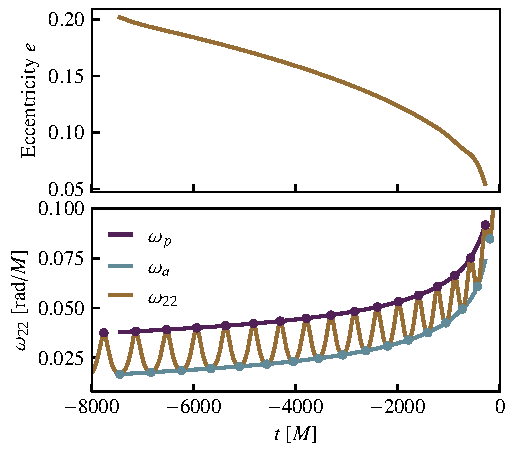
\includegraphics[width=\columnwidth]{ecc_definition}
    \label{fig:ecc_definition}
    \caption{Time evolution of the eccentricity $e(t)$ (upper panel) and the frequency of (2, 2) mode $\omega_{22}(t)$ (lower panel) for NR simulation (insert the simulation id here).
      $\omega_p(t)$ and $\omega_a(t)$ are spline interpolants of the frequency of (2, 2) mode at the pericenter and apocenter, respectively. The spine interpolants $\omega_p(t)$ ad $\omega_a(t)$
      are created using the values of $\omega_{22}$ at the pericenter (local maxima, deep violet circles) and the apocenter (local minima, cyan circles), respectively. The red dashed vertical line
      denotes the reference reference time $t_{\text{ref}}=-5500$ and red circle (upper panel) denotes the measured value of eccentricity at reference time.}
    \end{minipage}\hfill
    \begin{minipage}[t]{0.475\textwidth}
      \centering
      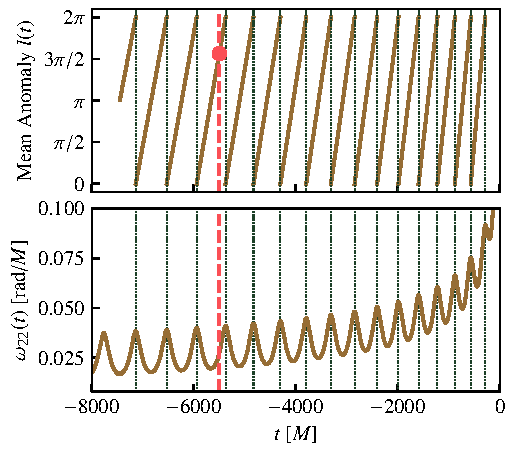
\includegraphics[width=\columnwidth]{mean_ano_definition}
      \label{fig:mean_anomaly_definition}
      \caption{Time evolution of the mean anomaly $l(t)$ (upper panel) and the $\omega_{22}(t)$ (lower panel). The vertical green dotted lines denote the local maxima (times of passage of pericenter). The mean anomaly varies linearly with time between two successive passages of pericenter. The slope of $l(t)$ becomes steeper as the binary inspirals due the reducing radial period. The red dashed line indicates the reference time $t_{\text{ref}}=-5500$ and the red circle (upper panel) denotes the measured value of the mean anomaly.}
    \end{minipage}
\end{figure*}

For an eccentric orbit, apart from the eccentricity, one can define another quantity called the mean anomaly $l(t)$. In the Newtonian context it is defined as
\begin{equation}
\label{eq:mean_anomaly_definition}
l(t) = 2\pi \frac{t - t_0}{P}
\end{equation}
where $t_0$ is the time of the last pericenter passage and $P$ is the radial period which is defined to be the time between two successive pericenter passages.
In the Newtonian case, the radial period $P$ is a constant but in general relativistic case, it changes as the binary inspirals.

%==========================================================================
\section{Measurement of eccentricity and mean anomaly}
\label{sec:measurement-of-eccentricity-and-mean-anomaly}
Given a gravitational waveform, we proceed to measure the eccentricity and mean anomaly at the desired reference time (or reference frequency) in the following three steps
\begin{enumerate}
\item Find the locations of the pericenter and apocenter and get the values of $\omega_{22}$ at the pericenter ($\omega_p$) and apocenter ($\omega_a$),
\item Construct spline interpolants $\omega_p(t)$ and $\omega_a(t)$ using the values of $\omega_{22}$ at the pericenter and apocenter, respectively, from the previous step,
\item Plug in $\omega_p(t)$ and $\omega_a(t)$ in (\ref{eq:eccentricity_definition}) to measure eccentricity. For mean anomaly, use the locations of pericenter from the first step to find the times of
  passage of pericenter and use those in (\ref{eq:mean_anomaly_definition}).
\end{enumerate}

%==========================================================================
\section{Implementation}
\label{sec:implementation}


%==========================================================================
\section{Tests}
\label{sec:tests}
To check the robustness of our eccentricity definition and the implementations using different methods, we put our implementations
through different tests. One of the checks for robustness of our implementation is to see how well it works for waveforms of eccentricities
varying from very low to high values. For this purpose, we generate hundreds of EOB waveforms using \texttt{SEOBNRv4EHM} model (cite Toni's paper) with eccentricity
(this is the eccentricity that the model takes as an input, we call this EOB eccentricity $e_{\text{EOB}}$) from $e_{\text{EOB}} = 10^{-7}$ to $e_{\text{EOB}} = 0.5$ keeping
other parameters (mass ratio and spins of the black holes) fixed. We do the following two tests using these waveforms

\subsection{EOB eccentricity vs measured eccentricity}
\label{sec:eob-eccentricity-vs-measured-eccentricity}
In this test, we compare the eccentricity that the EOB model takes as an input (the EOB eccentricity $e_{\text{EOB}}$) and the eccentricity that we measure using
our definition in (\ref{eq:eccentricity_definition}) at a specific reference time. For this test, we choose our reference time to be at the first available local
extremum (pericenter or apocenter). As we vary the $e_{\text{EOB}}$ smoothly from low to high values we expect the measured eccentricities to also vary smoothly.
This test also checks whether a particular implementation is able to measure the eccentricity at all. This is because, as $e_{\text{EOB}}$ becomes smaller and smaller
some of the implementations may fail to detect any local extrema and therefore can not measure eccentricity beyond a certain $e_{\text{EOB}}$. In \ref{fig:eob_vs_measured_ecc},
we show how the measured eccentricities varies with the EOB eccentricities for waveforms with $q=4, \chi_{1z}=-0.6, \chi_{2z}=-0.6$.


%--------------------------------------------------------------------------
\begin{figure}[thb]
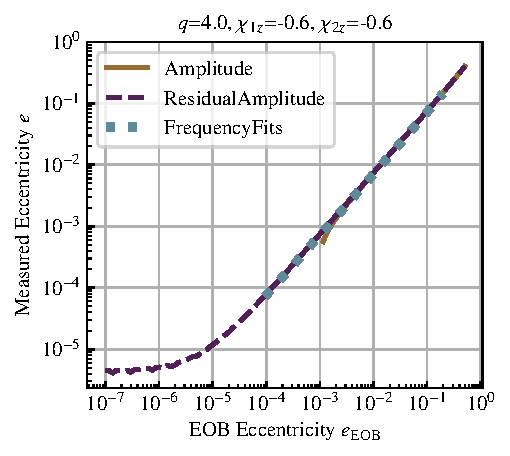
\includegraphics[width=\columnwidth]{test_eob_vs_measured_ecc_example}
\caption{EOB eccentricity vs measured eccentricity. This plot illustrates the capabilities and robustness of different methods to measure eccentricities from very low to high $e_{\text{EOB}}$.
  While all methods works nicely for relatively high eccentricities $e_{\text{EOB}} \gtrsim 10^{-2}$, \texttt{Frequency} and \texttt{Amplitude} methods start to deviate from others
  and fails to measure eccentricities as $e_{\text{EOB}}$ becomes close to $10^{-3}$. On the other hand the residual methods, \texttt{ResidualFrequency} and \texttt{ResidualAmplitude}
can measure eccentricities up to $e_{\text{EOB}} \simeq 10^{-5}$ and after that the measured eccentricities tend to saturate.}
\label{fig:eob_vs_measured_ecc}
\end{figure}

\subsection{Measured eccentricity vs time}
\label{sec:measured-eccentricity-vs-time}
In this test, we check how the evolution of measured eccentricity with time vary as we vary the EOB eccentricities for a given method. To make the visualization better,
we color the measured eccentricity vs time plots as a function of the $e_{\text{EOB}}$ and use a smoothly varying color gradient to choose the colors from. If a particular method
works for all $e_{\text{EOB}}$ from $10^{-7}$ to $0.5$ and for all the times upto the merger, then we expect the measured eccentricity vs time plots for that method to form a band of colors
smoothly varying from color of one end to the other end of the color gradient we are using. We also expect each line representing the evolution of measured eccentricity to be smooth and monotonically
decreasing.

\begin{figure}[thb]
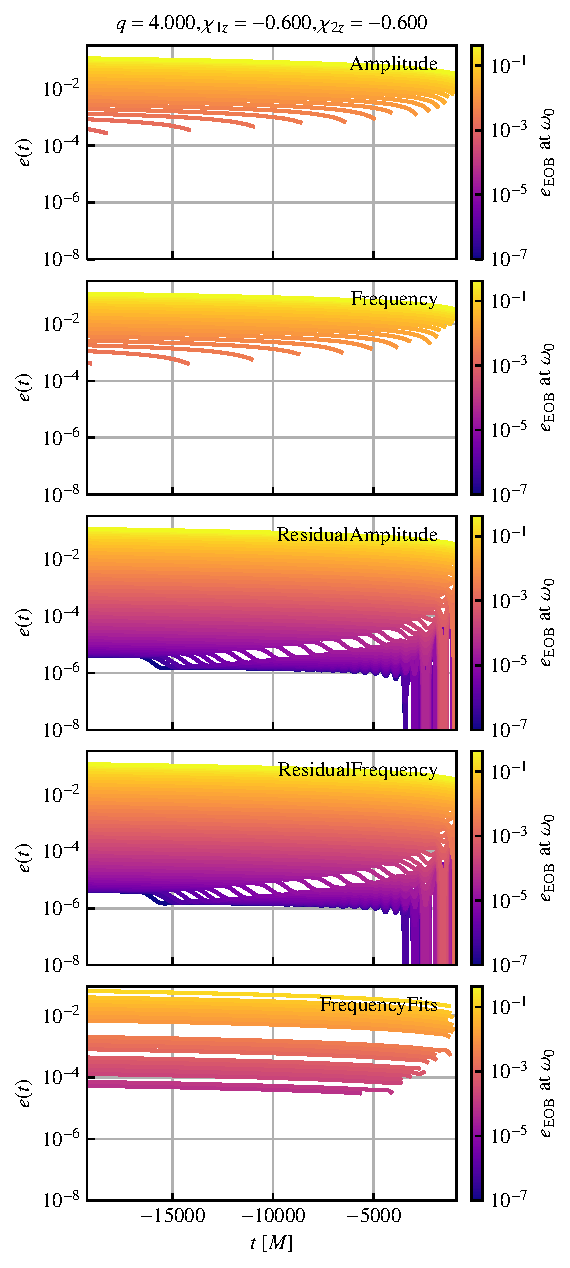
\includegraphics[width=\columnwidth]{test_measured_ecc_vs_time_example}
\caption{Evolution of measured eccentricity for varying $e_{\text{EOB}}$ for different methods. Text at top right corner indicates the method used. The colorbar on right indicates the $e_{\text{EOB}}$ of wavefomrs used to plot the evolution of measured eccentricity. \texttt{Amplitude} and \texttt{Frequency} methods work well upto $e_{\text{EOB}} \simeq 10^{-2}$ and below that the evolution stops further and further away from the merger. On ther other hand the \texttt{ResidualAmplitude} and \texttt{ResidualFrequency} methods work well upto $e_{\text{EOB}} \simeq 10^{-5}$ and the evolution goes all the way up to the merger. The sudden jump and the glitches we see in the evolution of the measured eccentricities for these two methods is due to the jump and glitches in $\omega_{22}$ data of the EOB waveform itself and not a drawback of the method itself (IMROVE THIS PHRASING).}
\label{fig:measured_ecc_vs_time}
\end{figure}

%==========================================================================
\section{Conclusion}
\label{sec:conclusion}
Here's what you should learn now that I done'd it.


%==========================================================================
\begin{acknowledgments}
% Randos
We thank Bob Loblaw for useful discussions.
% M.A.S
M.A.S.’s research was supported by the Department of Atomic Energy, Government of
India. M.A.S acknowledges travel support from Infosys Exchange Scholars program to visit
AEI, Potsdam and hospitality by AEI, Potsdam where a significant part of the work was
accomplished.
% V.V
V.V acknowledges support from the European Union’s Horizon 2020 research and
innovation program under the Marie Skłodowska-Curie grant agreement No.~896869.
% LIGO
This material is based upon work supported by NSF's LIGO Laboratory which is a
major facility fully funded by the NSF.
% GWOSC
%This research made use of data, software and/or web tools obtained from the
%Gravitational Wave Open Science Center~\cite{GW_open_science_center}, a service
%of the LIGO Laboratory, the LIGO Scientific Collaboration and the Virgo
%Collaboration.
\end{acknowledgments}

%%%%%%%%%%%%%%%%%%%%%%%%%%%%%%%%%%%%%%%%%%%%%%%%%%%%%%%%%%%%%%%%%%%%%%%%%%%%%%%
\section*{References}
%%%%%%%%%%%%%%%%%%%%%%%%%%%%%%%%%%%%%%%%%%%%%%%%%%%%%%%%%%%%%%%%%%%%%%%%%%%%%%%
\bibliography{References}


\end{document}
